\chapter{Implementation}\label{Implementation}

\blindtext









\section{Simulation}

\blindtext

\subsection{Virtualisation}

qemu+debvm
\blindtext

\begin{listing}[ht]
\inputminted{bash}{snippets/build.bash}
\caption[Building OpenSSL from source inside build.img with DebVM]{TODO builder}
\end{listing}

\subsection{Networking}

\blindtext

\begin{listing}[ht]
\inputminted{bash}{snippets/br0.bash}
\caption[Connecting QEMU virtual machines using a network bridge]{TODO br0}
\end{listing}

\blindtext

\begin{listing}[ht]
\inputminted{ini}{snippets/br0.ini}
\caption[Static bridge network configuration using systemd]{TODO /etc/systemd/network/00-br0.network contents}
\end{listing}

\blindtext

\begin{listing}[ht]
\inputminted{bash}{snippets/root.bash}
\caption[Generating a new self-signed root CA X.509 certificate using OpenSSL]{TODO root ca}
\end{listing}

\blindtext










\section{DNS Server}

\blindtext

\begin{listing}[ht]
\inputminted{bash}{snippets/dns.bash}
\caption[Signing a new X.509 certificate for ns.example.com using OpenSSL]{TODO dns}
\end{listing}

\blindtext

\begin{listing}[ht]
\inputminted{bash}{snippets/bind}
\caption[DNS over HTTPS configuration using BIND 9]{TODO /etc/bind/named.conf contents}
\end{listing}

\blindtext

\begin{listing}[ht]
\inputminted{zone}{snippets/example.zone}
\caption[Zone file for example.com zone with distributed ECH]{}
\end{listing}

\blindtext











\section{TLS Server}

\blindtext

\subsection{Peer Communication}

\blindtext

\begin{listing}[ht]
\inputminted{bash}{snippets/host_wg.bash}
\caption[Generating a new WireGuard key pair for tcd.example.com]{TODO host wg}
\end{listing}

\blindtext

\begin{listing}[ht]
\inputminted{ini}{snippets/host_wg.ini}
\caption[Configuring a WireGuard network interface using systemd]{TODO host wg}
\end{listing}

\begin{listing}[ht]
\inputminted{ini}{snippets/host_wg0.ini}
\caption[Static WireGuard network configuration using systemd]{TODO host wg0}
\end{listing}

\blindtext

\subsection{Web Server}

\blindtext

\begin{listing}[ht]
\inputminted{bash}{snippets/host_tls.bash}
\caption[Generating a new ECH key pair for tcd.example.com using OpenSSL]{TODO host+site tls}
\end{listing}

\blindtext

\begin{listing}[ht]
\inputminted{nginx}{snippets/nginx}
\caption[Distributed ECH NGINX configuration for tcd.example.com]{TODO nginx}
\end{listing}

\blindtext

\begin{listing}[ht]
\inputminted{bash}{snippets/padding.bash}
\caption[Rudimentary script to shroud legitimate WireGuard communication]{}
\end{listing}

\blindtext











\section{TLS Client}

\blindtext


\subsection{curl}

\blindtext

\begin{listing}[ht]
\inputminted{nginx}{snippets/curl.bash}
\caption[Command to use ECH-enabled curl on QEMU virtual machines]{TODO curl}
\end{listing}

\blindtext

\begin{figure}[ht]
\centerline{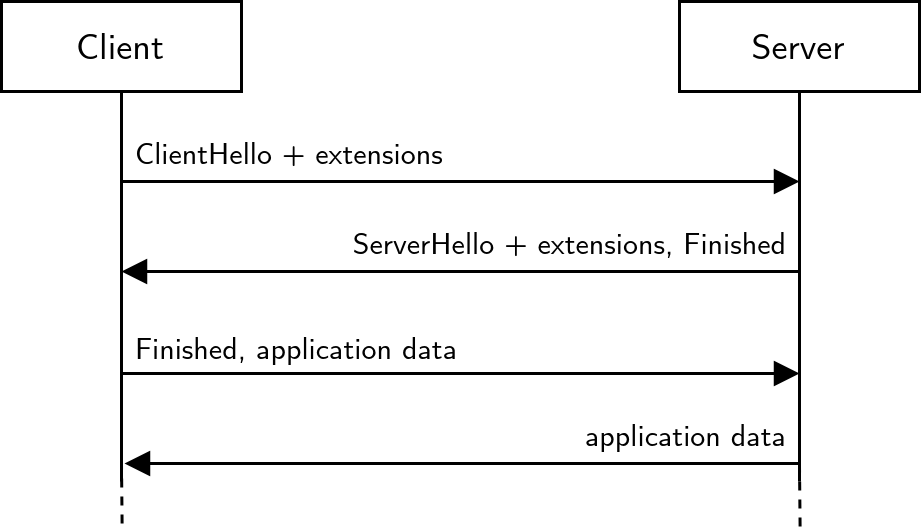
\includegraphics[width=120mm]{images/tls-handshake.png}}
\caption[Screenshot of curl output when accessing tcd.example.com]{<TODO>}
\label{curl_screenshot_figure}
\end{figure}

\subsection{Mozilla Firefox}

\blindtext

\begin{figure}[ht]
\centerline{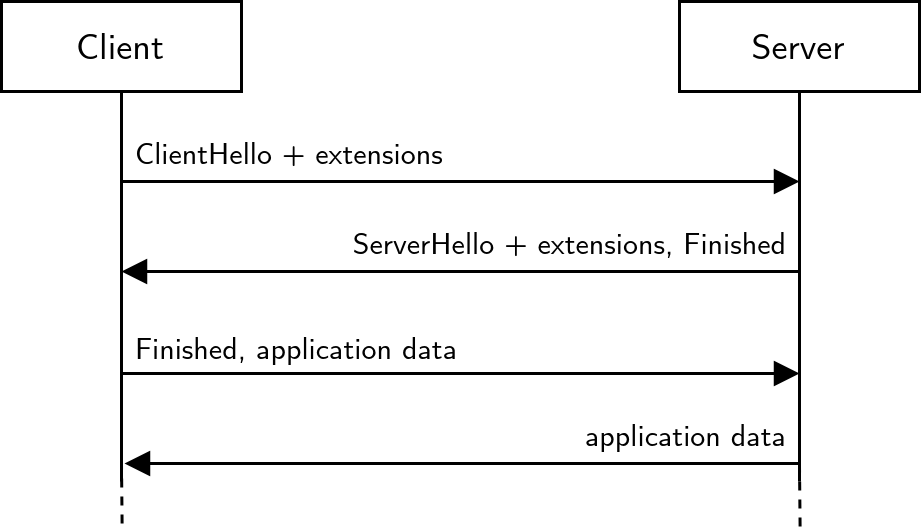
\includegraphics[width=120mm]{images/tls-handshake.png}}
\caption[Screenshot of Mozilla Firefox when accessing tcd.example.com]{<TODO>}
\label{firefox_screenshot_figure}
\end{figure}

\subsection{Google Chrome}

\blindtext

\begin{figure}[ht]
\centerline{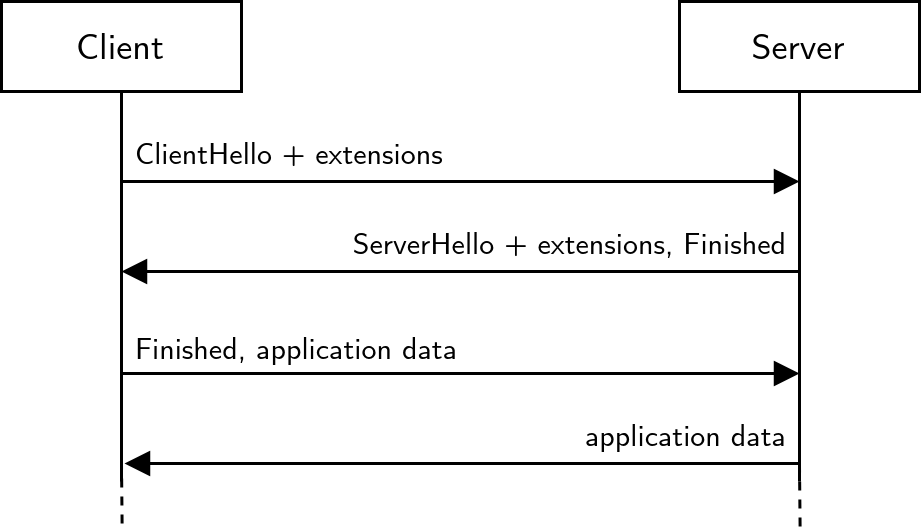
\includegraphics[width=120mm]{images/tls-handshake.png}}
\caption[Screenshot of Google Chrome when accessing tcd.example.com]{<TODO>}
\label{chrome_screenshot_figure}
\end{figure}











\section{Summary}

\blindtext
